\documentclass[10pt, border=3mm]{standalone}
\usepackage{pstricks-add}
\usepackage{tikz}
\usetikzlibrary{positioning, calc, graphs}
\renewcommand{\familydefault}{\sfdefault}

\begin{document}

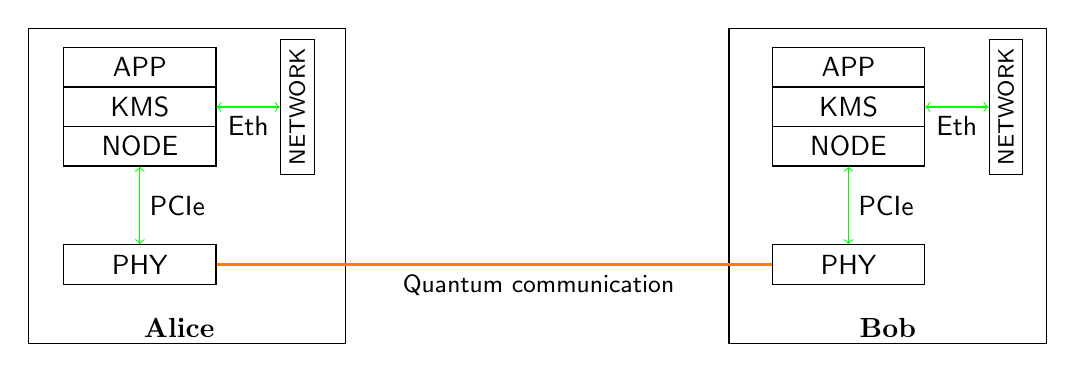
\begin{tikzpicture}[block/.style={rectangle,draw,minimum height=0.5cm,text width=1.7cm,align=center},node distance = 30mm, block2/.style={-, rectangle,draw,minimum height=4cm,text width=3.8cm,align=center} ]
\node (b1) [block] at (0,0) {PHY} ;
\node (b11) [block] at (0,1.5) {NODE};
\node (b12) [block] at (0,2) {KMS};
\node (b13) [block] at (0,2.51) {APP};
\node (b14) [draw] at (2,2) {\rotatebox{90}{\footnotesize{NETWORK}}};
\node (b15) [block2] at (0.6,1) {};
\node (b2) [block] at (9,0) {PHY};
\node (b21) [block] at (9,1.5) {NODE};
\node (b22) [block] at (9,2) {KMS};
\node (b23) [block] at (9,2.51) {APP};
\node (b24) [draw] at (11,2) {\rotatebox{90}{\footnotesize{NETWORK}}};
\node (b25) [block2] at (9.5,1) {};
  \begin{scope}
    \draw [<->, green] ([xshift=0cm]b1.north) -- ([xshift=0cm]b11.south) node [pos=0.5,right, black] {PCIe} ;
    \draw [<->, green] ([xshift=0cm]b2.north) -- ([xshift=0cm]b21.south) node [pos=0.5,right, black] {PCIe} ;
  \end{scope}
  \begin{scope}
   % \draw[double distance=20pt] (b1) -- node [sloped, above] {\small{Quantum channel }} (b2);
    \draw [-, orange, very thick] ($(b1.west)+(1.95,0)$) -- node [below, pos=0.58, black] {\small{Quantum communication }} ($(b2.east)+(-1.95,0)$);
    \draw [<->, green] ([yshift=0cm]b12) -- ([yshift=0cm]b14) node [below, pos=0.5, black] {Eth};
    \draw [<->, green] (b22) -- (b24) node [below, pos=0.5, black] {Eth};
    \node (input) at (0.5,-0.8){$\mathbf{Alice}$};
    \node (input) at (9.5,-0.8) {$\mathbf{Bob}$};
  \end{scope}
\end{tikzpicture}
\end{document}
